%--------
% Notes:
%   ~ADD       : Add the following.
%   ~REFERENCE : Reference the following paper/authors.
%   ~FIND      : Find a paper regarding the following.
%   ~CHECK     : Check that the following is met.
%   ~READ      : Read through the following paper/authors.
%   ~MENTION   : Mention the following.
%

\documentclass{UoYCSproject}
% Tikz Setup
\usepackage{tikz}
\usetikzlibrary{ matrix,      % For easy node positioning
                 fit,         % For easily fitting nodes inside another one
                 arrows,
                 positioning, % For easy node-relative placements
               }
\tikzstyle{edge} = [->, bend left]
\tikzstyle{vertex} = [circle, minimum width=0.5cm, text centered, draw=black]
\tikzstyle{graph} = [rectangle, draw=black, inner sep=1cm]
\tikzstyle{rule} = [rectangle, inner sep=1cm]
\tikzstyle{derivation} = [-implies, double]
% Listings Setup
\usepackage{listings}
\renewcommand{\lstlistingname}{C Code}

\author{Huw Taylor}
\title{Tracing and Debugging GP2}
\date{\today}
\supervisor{Dr. Detlef Plump}
\MEng
\wordcount
% ~CHECK: The bibTex reference LaTeX word count has the `accessed` field updated.
% ~16000 words (55 pages) total
\pagecount
\abstract{
% ~66 words
}
\acknowledgements{

}

\begin{document}

\maketitle
\tableofcontents
\listoffigures

\chapter{Introduction}
% ~1333 words
\section{Motivation}
The University of York has produced a graphical editor for creating graphs and graph programs. The editor depends on a compiler to produce the resultant graph, also made at the University of York. Both these tools are planned to be used by students in the coming academic year (2016/2017) for the GRAT module taught there.
The aim of this project is to show the intermediate steps of the programme, so that correctness of the compiler and the graphical editor can be ensured, and also so that students using these tools to learn how graph programmes work can see the process with a finer granularity.
\section{Ethics}
The project discussed has very few ethical considerations. It is not related to defence and there are no safety or security concerns.

\chapter{Literature Review}
% ~4000 words
% ~CHECK: Shows that you know what is happening in your field 
% ~CHECK: Justifies why your work is interesting or important 
% ~CHECK: establishes the theoretical framework/context for your work 
% ~CHECK: defends your choice of methodology 
% ~CHECK: avoids repeating previous researchers’ mistakes
\section{Graph Programming}
\subsection{Graph Transformations}
A graph is a visual way of representing data and relationships. The formal definition is a set of vertices (nodes) \emph{V}, a set of edges \emph{E}, and a set of labels \emph{L}. Additionally \emph{source} and \emph{target} functions associate edges with nodes, and a \emph{label} function, which maps labels to edges and nodes.
This field was first proposed in the 1970s by Ehrig, Pfender \& Schneider \cite{grat_origin}.
\emph{TO~ADD: briefly mention double-pushout/single-pushout methods and give graphical examples.} % ~ADD: references to double-pushout and single-pushout methods, as well as contributions to graph theory in general
The mathematical theory of Graph Transformation allows the transformation of graphs by way of rules. Rules are applied to graphs. They include a LHS (Left-Hand Side) graph, and RHS (Right-Hand Side) graph and an interface graph, which connects nodes in the LHS to nodes in the RHS. If the interface graph is ommited then it is inferred that it compises the common labelled nodes in both the LHS and RHS.

Figure \ref{fig:simple_rule} on page \pageref{fig:simple_rule} shows a simple rule that removes an edge. Note that nodes 1 and 2 can be the same node in the host graph, and so will remove edges whose source and target nodes are the same. Figure \ref{fig:simple_rule_sans_k} on page \pageref{fig:simple_rule_sans_k} shows the same rule without its interface graph.

\begin{figure}
\label{fig:simple_rule}
\centering
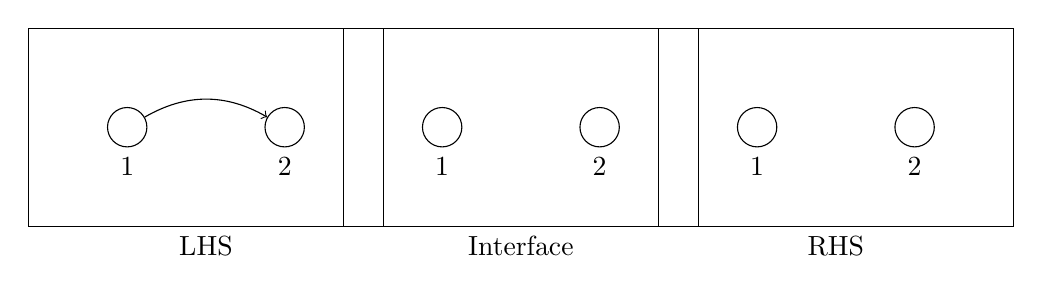
\begin{tikzpicture}[scale=2]
  \node (n1) [vertex, label=below:{1}] at (0, 0) {};
  \node (n2) [vertex, label=below:{2}] at (1, 0) {};
  \path [edge] (n1) edge node {} (n2);
  \node (l) [graph, fit={(n1) (n2)}, label=below:{LHS}] {};
  
  \node (n3) [vertex, label=below:{1}] at (2, 0) {};
  \node (n4) [vertex, label=below:{2}] at (3, 0) {};
  \node (k) [graph, fit={(n3) (n4)}, label=below:{Interface}] {};
  
  \node (n5) [vertex, label=below:{1}] at (4, 0) {};
  \node (n6) [vertex, label=below:{2}] at (5, 0) {};
  \node (r) [graph, fit={(n5) (n6)}, label=below:{RHS}] {};
\end{tikzpicture}
\caption{Rule Example}
\end{figure}

\begin{figure}
\label{fig:simple_rule_sans_k}
\centering
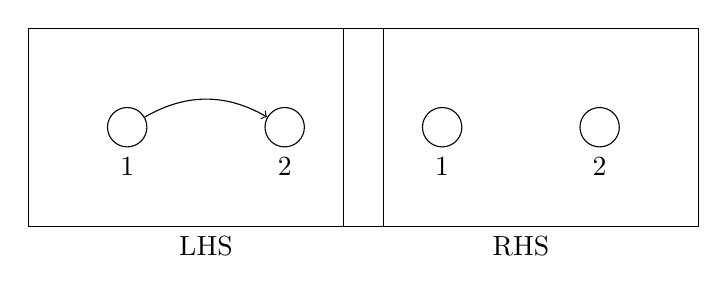
\begin{tikzpicture}[scale=2]
  \node (n1) [vertex, label=below:{1}] at (0, 0) {};
  \node (n2) [vertex, label=below:{2}] at (1, 0) {};
  \path [edge] (n1) edge node {} (n2);
  \node (l) [graph, fit={(n1) (n2)}, label=below:{LHS}] {};
  
  \node (n5) [vertex, label=below:{1}] at (2, 0) {};
  \node (n6) [vertex, label=below:{2}] at (3, 0) {};
  \node (r) [graph, fit={(n5) (n6)}, label=below:{RHS}] {};
\end{tikzpicture}
\caption{Rule Example without Interface Graph}
\end{figure}

% ~READ, ~ADD: https://www.cs.york.ac.uk/plasma/wiki/index.php?title=GP_%28Graph_Programs%29 Lots of relevant papers and a couple of example programs i can steal and reference.
\subsection{GP}
Graph Programming is XYZ
The University of York has developed a graph programming language \emph{GP} \cite{gp1}, and is developing a new implementation \emph{GP2}. The goal of both of these has been to write programs that manipulate graphs in terms of the graphs, rather than in general purpose languages like C or Java. The first GP was produced by Greg Manning. 
A GP allows the application of \emph{programs} to graphs. A program is made up of rules and rudimentary control structures, such as conditions, and loops. The rules are executed non-deterministically on a graph, known as the \emph{Host Graph}. The resulting graph is known as the \emph{Derived Graph}. A simple program could just be the continued application of a single rule.
\emph{TO~ADD: example of simple graph programs} % ~ADD: examples of simple graph programs illustrating calling rules (and the rules themselves), and loops, and

\begin{figure}
\label{fig:simple_program}
\centering
\begin{tikzpicture}[scale=2]
  \node (code) at (0, 1.5) {$main = RemoveEdge!;$};
  \node (rule_1) at (0, 1) {$RemoveEdge(a,b,c : int) = $};

  \node (n1) [vertex, label=below:{1}] at (0, 0) {a};
  \node (n2) [vertex, label=below:{2}] at (1, 0) {b};
  \path [edge] (n1) edge node[label=above:{c}] {} (n2);
  \node (l) [rule, fit={(n1) (n2)}] {};
  
  \node (n5) [vertex, label=below:{1}] at (2, 0) {a};
  \node (n6) [vertex, label=below:{2}] at (3, 0) {b};
  \node (r) [rule, fit={(n5) (n6)}] {};
  
  \draw[-implies,double, thick] (l) -- (r);

\end{tikzpicture}
\caption{Simple Graph Program}
\end{figure}


The original GP implementation is separated into four components:
\subsubsection{York Abstract Machine}
The YAM was written in C and focusses heavily on optimisation and performance, often sacrificing maintainability. It takes in the rules, represented in bytecode, and executes them on host graphs, on an abstract machine \cite[p. 13]{gp2_ide}.
% ~REFERENCE: Alex elliot paper page 14
\subsubsection{YAM Compiler}
The YAM Compiler compiles an XML representation of the graph program and its rules into YAM bytecode to be run on the abstract machine. It is written in Haskell.
\subsubsection{GXL to YAMG Converter}
YAMG is YAM's internal graph structure, and the converter takes in GXL, which is a subset of XML and a standard format for representing graphs.
\subsubsection{GP Editor}
The GP Editor was a GUI written in Java which allowed the creation of graphs graphically, as well as defining rules. It also displayed the derived graph.
The GP Editor has had very little thought of usability put into it\cite[p. 35]{gp_ge}. There are very few instructions to those intenting to use the tool, and the editor itself does little to help new users \cite[p. 44, 45]{gp_ui}.
% ~READ, ~MENTION: Zhang 2.3.2 (p31-32)

The main problem found with GP was that these components relied heavily upon each other, and documentation on how their interfaces are non-existent. % ~Spelling
This meant that all four components had to be regarded as a single system, which made alterations to any of them very difficult. This was the primary motivation behind GP2.

\subsection{GP2}
GP2 has a number of differences in the way in which it was implemented. As well as trying to address the issues of maintainability and usability, several features were added.
Instead of using an abstract machine, GP2 generates C code directly \cite{chris_compiler}, which removes the reliance on YAM, the YAM compiler, and YAM graph and program formats. It means that any C compiler can be used to generate the bytecode. It also attempts to standardise and document the format of graphs and programs that it takes. This means that tools to generate graphs either graphically or programmatically can be created without reducing modularity or creating complexity and interdependance between the components of the system \cite{gp2_ide}. % ~CHECK: This isn't bullshit

GP2 no longer enforces non-detereministic execution \cite[p. 15]{gp2_ide}, and doesn't backtrack to reach all possible solutions. This was done to achieve a higher level of implementation efficiency \cite[p. 15]{chris_compiler}, but sacrifices completeness.
\emph{TO~ADD: mention the haskell interpreter but say it's not `official'.} % ~MENTION: no longer non-deterministic. no backtracking and no longer the case that all solutions will be reached. Maybe mention the haskel one and its optional backtracking.

\subsection{GP2 Editor}
The GP2 graphical editor for creating graphs and graph programs is currently under development. It will allow for the creation of graphs graphically, rather than textually, and it will allow for the creation of programs textually, and their rules graphically, assigning the LHS and RHS of the rules. In contrast with the GP1 editor, the GP2 editor will also include functionality to highlight nodes.

\section{Tracing}
Tracing through the steps of a program has been around since programs themselves. % ~FIND: origins of tracing for debugging
It allows programmers to ensure that each step is procuding the right results and allows a more detailed insight into the workings of a program. Formal methods have been discussed as far back as the 70s \cite{psych_debug, code_walkthroughs}.

% ~FIND: some papers on debugging
% ~READ: psych_debug and code_walkthroughs for stuff to say about tracing/debugging
% ~READ: https://bitbucket.org/pypy/extradoc/src/tip/talk/pepm2011/bolz-allocation-removal.pdf (reference #16 might be good)


% END OF LITERATURE REVIEW

\chapter{Approach}
\section{Requirement Identification}
% ~2000 words
\begin{enumerate}
	\item Rules must be able to be stepped through one at a time.
 	\item The current rule must be made apparent graphically somehow.
	\item \ldots
\end{enumerate}
\section{Design}
% ~3333 words
\begin{itemize}
	\item Lifecycle
 	\item Engineering approach
 	\item Time management and/or general plan
	\item \ldots
\end{itemize}
 
\subsection{Tools}
Not a lot really.
\begin{itemize}
  \item Git
  \item Some C compiler/IDE/something or another
  \item Dependencies for GP-Editor
  \item \ldots
\end{itemize}
\section{Implementation}


\begin{lstlisting}[label=c_1, caption=Placeholder C Code]
*foo = &bar;
\end{lstlisting}


\chapter{Evaluation}
% ~3333 words
\chapter{Conclusions}
% ~1333 words
\section{Future Work}

% \bibliography{references}

\chapter{Appendices}
\end{document}